\section{Serial Input/Output}
\subsection{Datenübermittlung}
Digitale Signale lassen sich sehr schlecht auf analogen Leitungen übertragen, daher werden die Signale auf einen Träger moduliert.
\begin{itemize}
  \item Amplituden Modulation (AM)
  \item Frequenz Modulation (FM)
  \item Phasen Modulation (PM)
\end{itemize}

Der Übertragungskanal kann verschieden aufgebaut sein, man unterscheidet:
\begin{itemize}
  \item \textbf{Simplex:} Nur eine Leitung. Nur einer kann senden, der andere kann nur empfangen.
  \item \textbf{Halb-Duplex:} Eine Leitung, aber beide können senden und empfangen, jedoch nicht zur gleichen Zeit
  \item \textbf{Voll-Duplex:} Zwei Leitungen, beide können jederzeit senden und empfangen.
\end{itemize}

\subsubsection{Übertragungsgeschwidigkeit}
\begin{itemize}
  \item \textbf{Baud Rate: (Baud)} Anzahl Zustände pro Sekunde
  \item \textbf{Bits pro Sekunde: (BPS)} Anzahl Informationen welche pro Sekunde übermittelt werden können
\end{itemize}
Baud und BPS sind nicht dasselbe! Für ein binäres zwei-Level Signal mit der Datenrate 1 BPS ist die Baud 1.
Ein Signal mit 16 diskreten Level kann pro Zustand 4 ($16=2^4$) Bit übermitteln. Bei einer Baud von 1200 sind das also 4800 BPS! 

\subsection{Asynchrone vs. Synchrone Übermittlung}
\begin{tabular}{ll}
	\textbf{Asynchron:}	& Jedes übermittelte Zeichen hat framing bits, welche den Beginn und das Ende markieren \\
	\textbf{Synchron:}	& Es werden Datenblöcke übermittelt, welche von framing	bits umgeben sind.
\end{tabular}

\subsection{RS-232}
\subsubsection{Signalverlauf}
  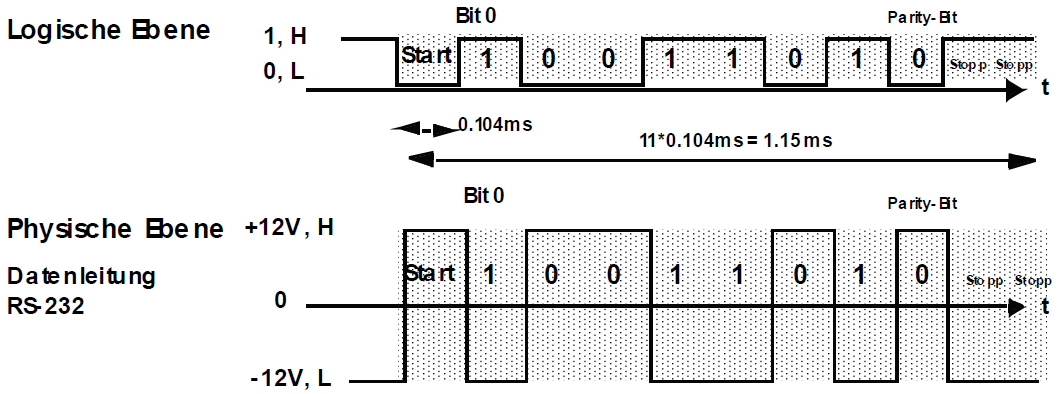
\includegraphics[width= 12cm, height=3cm]{pictures/RS2323_Signalverlauf}
  \begin{itemize}
    \item Das Paritätsbit bewirkt, dass bei gerader („EVEN“) Parität immer eine
    gerade bzw. bei ungerader („ODD“) Parität eine ungerade Anzahl von „1“-Bits übertragen wird. Es gibt also die Möglichkeiten „E“ wie even parity oder „O“ wie odd parity oder kein Parity-Bit entsprechend „N“ wie no parity. Weiterhin kann das Paritätsbit immer gesetzt („M“ wie mark parity) oder immer gelöscht („S“ wie space parity) sein. Abgeschlossen wird die Übertragung mit ein oder zwei Stoppbits logisch „1“
    \item Das LSB wird zuerst geschickt
  \end{itemize}
\subsubsection{Datenleitungen}
\begin{tabular}{|l|l|p{12cm}|}
  \hline
  \textbf{Abkürzung} & \textbf{Name} & \textbf{Beschreibung}\\ \hline
  TxD, TX, TD & Transmit Data & Leitung für ausgehende (von DTE gesendete) Daten
  (negative Logik)\\ 
  \hline
  RxD, RX, RD & Receive Data & Leitung für eingehende (von DTE zu empfangende)
  Daten (negative Logik).\\ 
  \hline
  RTS & Request to Send & „Sendeanforderung“; Ein High-Pegel an diesem Ausgang
  signalisiert, dass DTE Daten senden möchte.\\
  \hline
  CTS & Clear to Send & „Sendeerlaubnis“; Ein High-Pegel an diesem Eingang ist
  ein Signal der Gegenstelle, dass sie Daten von DTE entgegennehmen kann.\\
  \hline
  DSR & Data Set Ready & Ein High-Pegel an diesem Eingang ist ein Signal der
  Gegenstelle, dass sie im Prinzip einsatzbereit ist (aber nicht
  notwendigerweise auch empfangsbereit, siehe CTS)\\
  \hline
  DCD, CD, RLSD & (Data) Carrier Detect & Mit einem High-Pegel an diesem Eingang
  signalisiert die Gegenstelle, dass sie einlaufende Daten auf der Leitung
  erkennt (dem Namen nach ist das die Modulationsträger-Erkennung) und an DTE
  weitergeben möchte.\\
  \hline
  DTR & Data Terminal Ready & Mit einem High-Pegel an diesem Ausgang
  signalisiert DTE seine Betriebsbereitschaft an die Gegenstelle. Damit kann die
  Gegenstelle, z. B. ein Modem, aktiviert oder auch zurückgesetzt werden.
  Üblicherweise antwortet die Gegenstelle mit einem High-Pegel auf DSR.\\
  \hline
  RI & Ring Indicator & Ein High-Pegel an diesem Eingang signalisiert dem
  DTE-Gerät, dass ein Anruf ankommt, d.h. dass jemand eine Datenverbindung
  aufzubauen wünscht, („ring“ ist engl. für „klingeln“; besonders bei Telefonen
  und im übertragenen Sinne auch bei Modems).\\ 
  \hline
  
\end{tabular}